Normalerweise wird Java in einem zweistufigen Prozess ausgeführt. Zunächst wird eine plattformabhängige JVM geladen. Innerhalb dieser JVM wird der Java-Compiler (javac) aufgerufen. Dieser compiliert Java-Quelltext zu Java-Bytecode. Der Java-Bytecode kann dann von der JVM ausgeführt werden. Dieser Ablauf ist in der \ref{abb:java_execution} unter a) dargestellt.

Um Java in einem Browser auszuführen ergeben sich konzeptionell mindestens drei verschiedene Möglichkeiten, die in \ref{Abbildung 4.4} mit den Buchstaben b-d gekennzeichnet sind.

\begin{figure}[H]
    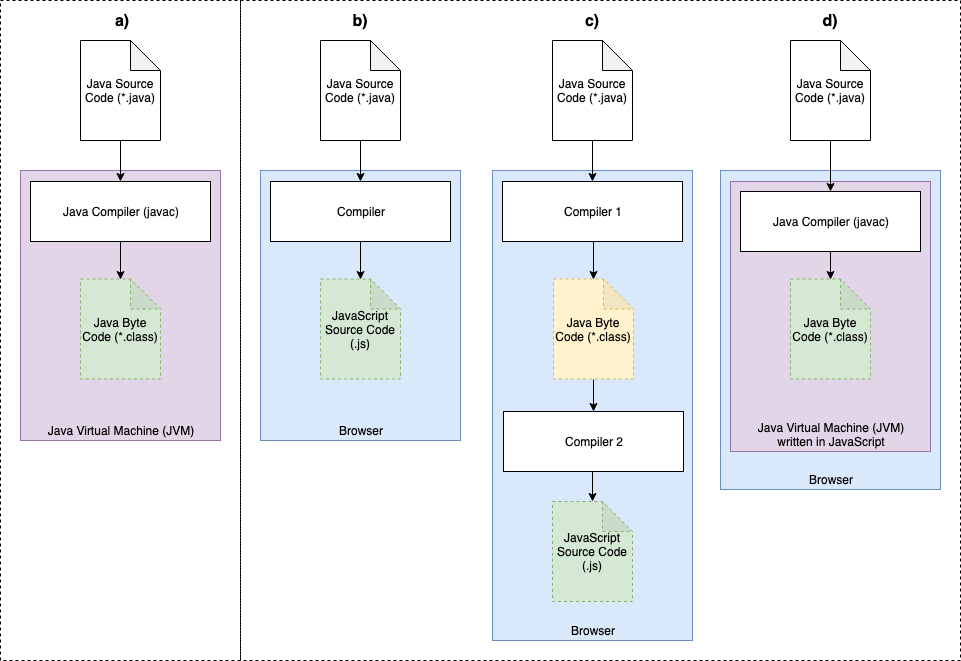
\includegraphics[width=14cm]{chapter/entwurf/bilder/Java_JavaScript_Execution.png}
    \centering
    \caption{Blubb}
    \label{abb:java_execution}
\end{figure}

\begin{itemize}
    \item \textbf{b:} Java-Quelltext wird mit einem Compiler direkt in JavaScript umgewandelt: Diese Variante ist konzeptionell sehr einfach. Zwar gibt es einige Programme, welche Java-Quelltext in JavaScript übersetzen können (zum Beispiel JSweet oder GWT), jedoch sind alle diese Programme entweder in Java selbst oder in anderen Programmiersprachen verfasst. Einen solchen Compiler, der selbst in JavaScript geschrieben wurde, gibt es bisher nicht. Es wäre möglich eines der besagten Programme auf einem separaten Server zu verwenden. Dies würde aber eine weitere Abhängigkeit von einem Server bedeuten, und damit der formulierten Kern-Anforderung widersprechen.
    \item \textbf{c:} Java-Quelltext wird mithilfe eines ersten Compilers in Java-Bytecode übersetzt. Anschließend wird der Java-Bytecode mit einem zweiten Compiler in JavaScript übersetzt. Auch hier ergibt sich das gleiche Problem wie in b). Zwar gibt es Programme, die den jeweiligen Teilschritt übernehmen könnten, jedoch ist keins davon in JavaScript verfasst, so dass es keine Lösung dafür im Browser gibt.
    \item \textbf{d:} Es wird eine JVM verwendet, die in JavaScript implementiert wurde. Mithilfe dieser JVM kann der javac-Compiler geladen werden, um Java-Quelltext in Java-Bytecode zu übersetzen und anschließend auszuführen. Eine solche JavaScript-JVM existiert bereits in Form eines Universitätsprojekt der University of Massachusetts unter dem Namen DoppioJVM. Der konzeptionelle Nachteil dieser Lösung liegt in der benötigten Datenmenge: Um eine komplette JVM im Browser auszuführen wird ebenfalls die Java Runtime Environment benötigt, deren Größe bei etwa 60 Megabyte liegt.
\end{itemize}

In Anbetracht der Tatsache, dass die Ausführung der Code-Beispiele im Browser exakt die gleichen Ergebnisse liefern soll, wie die Ausführung in einer lokalen JVM (zum Beispiel auch in Bezug auf Fehler beim Kompilieren), so ist die Variante d die bevorzugte Lösung und wurde im Rahmen dieser Arbeit in das entstandene CRS integriert.

DoppioJVM ist das Ergebnis der PLASMA-Forschungsgruppe der University of Massachusetts in Amherst, USA. Das Projekt wurde im Jahr 2014 im Rahmen einer wissenschaftlichen Arbeit veröffentlicht und wird von den Autoren selbst wie folgt beschrieben:

\begin{quotation}
„DoppioJVM is a robust prototype Java Virtual Machine (JVM) interpreter
that operates entirely in JavaScript. DoppioJVM implements all
201 bytecode instructions specified in the second edition of the
Java Virtual Machine Specification, supports multithreaded
programs, runs multiple languages that run on top of the JVM, and
implements many of the complex mechanisms and native functionality that JVM programs expect.“
\end{quotation}

Voraussetzung für den Betrieb von DoppioJVM ist ein weiteres Projekt der gleichen Forschungsgruppe: BrowserFS. Dabei handelt es sich um die Implementation eines NodeJS-kompatiblen Dateisystems innerhalb des Browsers. Somit können JavaScript-Programme, die eigentlich für die NodeJS-Laufzeitumgebung gestaltet sind (also Zugriffe auf ein Dateisystem ermöglichen) auch im Browser ausgeführt werden. BrowserFS emuliert ein Dateisystem auf Basis verschiedener Webstandards. So können für den Betrieb der DoppioJVM zum Beispiel die JRE-Komponenten über ein virtuelles Dateisystem bereitgestellt werden, welches auf dem asynchronen Nachladen basiert, oder andere Komponenten der JVM über den LocalStorage des Browsers.

Nachdem das BrowserFS-Dateisystem konfiguriert ist, kann DoppioJVM mit einer relativ einfachen Schnittstelle verwendet werden:

\begin{minipage}{\linewidth}
\begin{lstlisting}
new Doppio.VM.JVM(
  {
    doppioHomePath: "/sys",
    classpath: [".", "/sys/", "/tmp/"]
  },
  (err, jvmObject) => {
    jvmObject.runClass("Loader", [classname], exitCode => {
      if (exitCode !== 0) {
        console.log("JVM exited with an error");
      } else {
        console.log("JVM exited successfully");
      }
    });
  }
);
\end{lstlisting}
\end{minipage}

Die DoppioJVM muss bei jeder Verwendung neu instantiiert werden. Deswegen ist es erforderlich, dass die Kompilierung und Ausführung des gewünschten Java-Codes in einem Aufruf erfolgt. Dazu hat Java einige Möglichkeiten an Bord, die in Form der folgenden Loader-Klasse implementiert wurden:

\begin{minipage}{\linewidth}
\begin{lstlisting}
import javax.tools.*;
import java.lang.reflect.*;
import java.io.*;
import java.net.*;

public class Loader {
  public static void main(String[] args) {
    if (args.length == 0) {
      System.out.println("No class was found.");
      System.exit(1);
    }
    String className = args[0];
    String sourceFile = "/tmp/" + className + ".java";
    String classFile = "/tmp/" + className + ".class";

    System.out.println("Compiling found class '" + className + "'...");

    JavaCompiler compiler = ToolProvider.getSystemJavaCompiler();
    int result = compiler.run(null, null, null, sourceFile, "-d", "/tmp/");

    if (result == 0) {
      try {
        System.out.println("Compilation successful. Executing...");
        System.out.println("---");

        URLClassLoader classLoader = new URLClassLoader(
            new URL[] {new File(classFile).toURI().toURL()}, ClassLoader.getSystemClassLoader());
        Class<?> c = classLoader.loadClass(className);
        Method m = c.getDeclaredMethod("main", String[].class);
        m.invoke(null, new Object[] {});
        classLoader.close();

        System.out.println("Execution successfull");
      } catch (Exception e) {
        e.printStackTrace();
      }
    } else {
      System.out.println("Could not compile");
    }
  }
}
\end{lstlisting}
\end{minipage}